\documentclass{beamer}
\usetheme{Madrid}
\usecolortheme{dolphin}
\usepackage{graphicx}
\usepackage{hyperref}
\usepackage{listings}
\usepackage{tikz}

\title{Identity and Access Management}
\subtitle{Securing Systems in the Digital Age}
\author{Instructor Name}
\institute{School/College Name}
\date{\today}

\begin{document}

\begin{frame}
    \titlepage
\end{frame}

\begin{frame}{Welcome to Identity and Access Management: Securing the Digital Front Door}
    \begin{itemize}
        \item \textbf{Identity and Access Management (IAM)} is the framework for ensuring the right individuals access the right resources at the right times for the right reasons.
        \item Understanding IAM is essential for protecting systems against unauthorized access and potential security breaches.
        \item Modern organizations typically manage thousands of digital identities, making systematic approaches necessary.
        \item IAM encompasses both technical systems and policies that govern how identities are created, verified, and granted permissions.
    \end{itemize}
    
    \begin{alertblock}{Key Question}
        How do we ensure only authorized users can access sensitive information while still making systems convenient to use?
    \end{alertblock}
\end{frame}

\begin{frame}{Why IAM Matters: Real-World Security Scenarios}
    \begin{itemize}
        \item A hospital must ensure patient records are only accessible to authorized healthcare providers while maintaining ease of access in emergencies.
        \item Financial institutions need to verify identities before allowing transfers, with higher security requirements for larger transactions.
        \item Companies must immediately remove access when employees leave to prevent security vulnerabilities from lingering accounts.
        \item Educational institutions must provide appropriate access levels to students, faculty, and staff while protecting sensitive data.
    \end{itemize}
    
    \begin{example}
        The 2020 SolarWinds breach occurred partly because attackers gained privileged access credentials, showing how IAM failures can have devastating consequences across thousands of organizations.
    \end{example}
\end{frame}

\begin{frame}{The IAM Lifecycle: An Overview}
    \begin{itemize}
        \item The \textbf{IAM lifecycle} begins with identity creation and verification to establish who a user is.
        \item Once verified, users receive appropriate access permissions based on their role and needs.
        \item Throughout the lifecycle, authentication mechanisms verify user identity during each access attempt.
        \item The cycle concludes with de-provisioning when access is no longer needed or appropriate.
    \end{itemize}
    
    \begin{center}
        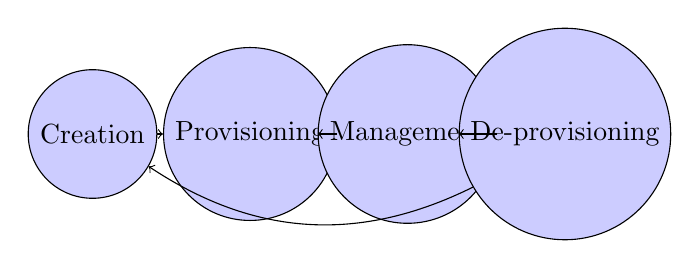
\begin{tikzpicture}
            \node[draw, circle, fill=blue!20] (a) at (0,0) {Creation};
            \node[draw, circle, fill=blue!20] (b) at (2,0) {Provisioning};
            \node[draw, circle, fill=blue!20] (c) at (4,0) {Management};
            \node[draw, circle, fill=blue!20] (d) at (6,0) {De-provisioning};
            
            \draw[->] (a) -- (b);
            \draw[->] (b) -- (c);
            \draw[->] (c) -- (d);
            \draw[->] (d) to[bend left] (a);
        \end{tikzpicture}
    \end{center}
\end{frame}

\begin{frame}{User Account Basics: Creating and Managing Digital Identities}
    \begin{itemize}
        \item A \textbf{digital identity} is the electronic representation of a person or entity within a system.
        \item User accounts store essential identifying information such as username, contact details, and authentication credentials.
        \item Most systems use unique identifiers (like user IDs) that remain consistent even when other account details change.
        \item Properly structured user accounts enable appropriate access while maintaining security and accountability.
    \end{itemize}
    
    \begin{block}{Components of a Digital Identity}
        \begin{itemize}
            \item Identifiers (username, email, ID number)
            \item Authentication data (password hash, biometric templates)
            \item Profile information (name, department, contact info)
            \item Access rights and permissions
        \end{itemize}
    \end{block}
\end{frame}

\begin{frame}{The Art of Provisioning: Adding Users Securely}
    \begin{itemize}
        \item \textbf{Provisioning} is the process of creating user accounts and assigning appropriate access rights to resources.
        \item Automated provisioning reduces human error and ensures consistency in how accounts are created and configured.
        \item Proper provisioning includes verification of identity before granting access to sensitive systems.
        \item Organizations typically develop standardized workflows to ensure all necessary approvals are obtained before access is granted.
    \end{itemize}
    
    \begin{table}
        \begin{tabular}{|l|l|}
            \hline
            \textbf{Provisioning Type} & \textbf{Best Used For} \\
            \hline
            Manual & Small organizations, specialized roles \\
            Self-service & Common resources, low-risk assets \\
            Automated & Large organizations, standard onboarding \\
            Just-in-time & Temporary access needs \\
            \hline
        \end{tabular}
    \end{table}
\end{frame}

\begin{frame}{De-provisioning: Why Removing Access Matters}
    \begin{itemize}
        \item \textbf{De-provisioning} is the systematic removal of access rights when they are no longer needed or authorized.
        \item Orphaned accounts (accounts belonging to former employees) represent significant security vulnerabilities if not properly managed.
        \item Effective de-provisioning should be timely, complete, and documented to maintain security compliance.
        \item Regular access reviews help identify accounts that should be de-provisioned but might have been overlooked.
    \end{itemize}
    
    \begin{alertblock}{Security Risk}
        The 2020 IBM Cost of a Data Breach Report found that organizations with orphaned accounts experienced higher data breach costs, with abandoned credentials frequently exploited by attackers.
    \end{alertblock}
\end{frame}

\begin{frame}{Identity Proofing: Verifying Who's Who}
    \begin{itemize}
        \item \textbf{Identity proofing} is the process of verifying that a person is who they claim to be before creating their digital identity.
        \item The strength of identity proofing should match the sensitivity of the resources the user will access.
        \item Common methods include document verification (ID cards, passports), knowledge-based verification, and biometric matching.
        \item The National Institute of Standards and Technology (NIST) defines three assurance levels for identity proofing, from basic to highly secure.
    \end{itemize}
    
    \begin{center}
        \begin{tabular}{|c|c|c|}
            \hline
            \textbf{IAL1} & \textbf{IAL2} & \textbf{IAL3} \\
            \hline
            Self-assertion & ID verification & In-person proofing \\
            No validation & Remote or in-person & Physical biometrics \\
            Minimal assurance & Moderate assurance & High assurance \\
            \hline
        \end{tabular}
    \end{center}
\end{frame}

\begin{frame}{Understanding Permissions: The Building Blocks of Access}
    \begin{itemize}
        \item \textbf{Permissions} are specific authorizations that allow users to perform particular actions on resources.
        \item Common permission types include read, write, execute, modify, and delete capabilities.
        \item Permissions can be assigned directly to users or indirectly through groups, roles, or attributes.
        \item Well-designed permission structures balance security needs with usability concerns.
    \end{itemize}
    
    \begin{block}{CRUD Permissions Model}
        Most systems organize permissions around four basic operations:
        \begin{itemize}
            \item \textbf{C}reate: Ability to generate new data or resources
            \item \textbf{R}ead: Ability to view existing data
            \item \textbf{U}pdate: Ability to modify existing data
            \item \textbf{D}elete: Ability to remove data or resources
        \end{itemize}
    \end{block}
\end{frame}

\begin{frame}{Permission Assignment: Who Gets What Access and Why}
    \begin{itemize}
        \item Permission assignment should be based on legitimate business needs rather than convenience or hierarchy.
        \item \textbf{Segregation of duties} ensures that critical functions are divided among different individuals to prevent fraud.
        \item Permissions can be assigned through static methods (manual assignment) or dynamic methods (calculated at access time).
        \item Regular permission audits help identify and correct inappropriate access rights before they cause security incidents.
    \end{itemize}
    
    \begin{example}
        A financial system might require two different employees to create and approve payment transactions, preventing any single individual from both creating and authorizing fraudulent payments.
    \end{example}
\end{frame}

\begin{frame}{The Principle of Least Privilege: Need-to-Know Access}
    \begin{itemize}
        \item The \textbf{principle of least privilege} states that users should be given only the minimum access rights needed to perform their job functions.
        \item Implementing least privilege reduces the potential damage from compromised accounts or insider threats.
        \item This principle applies to both human users and system processes or applications.
        \item Temporary privilege elevation can be used when higher-level access is occasionally needed but not justified permanently.
    \end{itemize}
    
    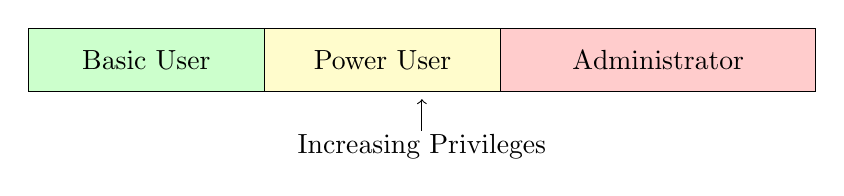
\begin{tikzpicture}
        \draw (0,0) rectangle (10,0.8);
        \draw[fill=green!20] (0,0) rectangle (3,0.8);
        \draw[fill=yellow!20] (3,0) rectangle (6,0.8);
        \draw[fill=red!20] (6,0) rectangle (10,0.8);
        
        \node at (1.5,0.4) {Basic User};
        \node at (4.5,0.4) {Power User};
        \node at (8,0.4) {Administrator};
        
        \draw[->] (5,-0.5) -- (5,-0.1);
        \node at (5,-0.7) {Increasing Privileges};
    \end{tikzpicture}
\end{frame}

\begin{frame}{Access Control Models: Different Approaches to Security}
    \begin{itemize}
        \item \textbf{Access control models} provide structured frameworks for determining who can access what resources.
        \item Different models address varying security needs, organizational structures, and compliance requirements.
        \item Most modern systems implement hybrid approaches that combine elements from multiple access control models.
        \item The choice of access control model significantly impacts both security posture and administrative complexity.
    \end{itemize}
    
    \begin{table}
        \begin{tabular}{|l|l|}
            \hline
            \textbf{Access Control Model} & \textbf{Key Characteristic} \\
            \hline
            Mandatory (MAC) & System-enforced based on sensitivity labels \\
            Discretionary (DAC) & Owner-determined access permissions \\
            Role-based (RBAC) & Access based on job functions/roles \\
            Rule-based & Access based on predefined rules \\
            Attribute-based (ABAC) & Dynamic access based on attributes \\
            \hline
        \end{tabular}
    \end{table}
\end{frame}

\begin{frame}{Mandatory vs. Discretionary Access Control: Understanding the Differences}
    \begin{itemize}
        \item \textbf{Mandatory Access Control (MAC)} uses system-enforced security labels that cannot be altered by users.
        \item MAC assigns sensitivity labels to resources and clearance levels to users, with access granted only when clearance meets or exceeds sensitivity.
        \item \textbf{Discretionary Access Control (DAC)} allows resource owners to determine who can access their resources.
        \item DAC is more flexible but potentially less secure, as permissions are at the discretion of individual users.
    \end{itemize}
    
    \begin{block}{When to Use Each Model}
        \begin{itemize}
            \item \textbf{MAC}: Military systems, government classified information, highly regulated industries
            \item \textbf{DAC}: Collaborative environments, file sharing systems, situations requiring user autonomy
        \end{itemize}
    \end{block}
\end{frame}

\begin{frame}{Role-Based Access Control: Organizing Permissions by Job Function}
    \begin{itemize}
        \item \textbf{Role-Based Access Control (RBAC)} assigns permissions to roles, and roles to users based on their job responsibilities.
        \item RBAC simplifies administration by managing permissions at the role level rather than individually for each user.
        \item When employees change positions, administrators need only assign them to different roles rather than reconfiguring all permissions.
        \item Roles can be hierarchical, allowing permissions to be inherited from more general to more specific job functions.
    \end{itemize}
    
    \begin{center}
        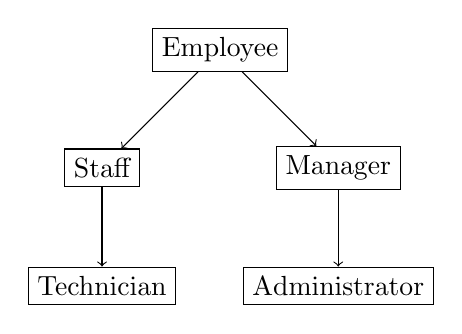
\begin{tikzpicture}[node distance=1.5cm]
            \node[draw, rectangle] (emp) {Employee};
            \node[draw, rectangle, below of=emp, left of=emp] (staff) {Staff};
            \node[draw, rectangle, below of=emp, right of=emp] (manager) {Manager};
            \node[draw, rectangle, below of=staff] (tech) {Technician};
            \node[draw, rectangle, below of=manager] (admin) {Administrator};
            
            \draw[->] (emp) -- (staff);
            \draw[->] (emp) -- (manager);
            \draw[->] (staff) -- (tech);
            \draw[->] (manager) -- (admin);
        \end{tikzpicture}
    \end{center}
\end{frame}

\begin{frame}{Rule-Based and Attribute-Based Access: Dynamic Security Controls}
    \begin{itemize}
        \item \textbf{Rule-Based Access Control} uses predefined rules to determine access permissions based on specific conditions.
        \item Rules can incorporate factors such as time of day, network location, or previous access patterns.
        \item \textbf{Attribute-Based Access Control (ABAC)} makes access decisions based on attributes of users, resources, actions, and environment.
        \item ABAC offers more granular control than RBAC but requires more complex policy definition and evaluation.
    \end{itemize}
    
    \begin{alertblock}{ABAC Policy Example}
        IF user.department = "Finance" AND resource.type = "Financial Report" AND action = "view" AND environment.time BETWEEN "9:00" AND "17:00" THEN permit
    \end{alertblock}
\end{frame}

\begin{frame}{Time-Based Restrictions: When Access Matters}
    \begin{itemize}
        \item \textbf{Time-based access restrictions} limit when users can access resources, regardless of their identities or roles.
        \item Time restrictions help prevent unauthorized access outside normal business hours when legitimate use is unlikely.
        \item These controls can be used to enforce maintenance windows, scheduled system upgrades, or compliance with labor regulations.
        \item Effective time-based controls must account for different time zones, holidays, and emergency access procedures.
    \end{itemize}
    
    \begin{table}
        \begin{tabular}{|l|p{7cm}|}
            \hline
            \textbf{Time Restriction Type} & \textbf{Use Case} \\
            \hline
            Hours of operation & Limiting access to business applications to normal working hours (8am-6pm) \\
            Day of week & Restricting system maintenance tasks to weekends only \\
            Date range & Allowing temporary contractors access only during their contract period \\
            Seasonal & Enabling tax filing systems only during tax season \\
            \hline
        \end{tabular}
    \end{table}
\end{frame}

\begin{frame}{Authentication 101: Proving Identity in the Digital World}
    \begin{itemize}
        \item \textbf{Authentication} is the process of verifying that a user is who they claim to be when accessing a system.
        \item Authentication is distinct from authorization, which determines what an authenticated user is allowed to do.
        \item Strong authentication typically relies on multiple factors rather than a single piece of evidence.
        \item Authentication strength should be proportional to the sensitivity of the information or systems being protected.
    \end{itemize}
    
    \begin{block}{Authentication vs. Authorization}
        \begin{itemize}
            \item \textbf{Authentication} answers: "Are you who you say you are?"
            \item \textbf{Authorization} answers: "What are you allowed to do?"
            \item Both are required for a complete access control system
        \end{itemize}
    \end{block}
\end{frame}

\begin{frame}{Password Best Practices: Length, Complexity, and Management}
    \begin{itemize}
        \item \textbf{Passwords} remain the most common authentication method despite their known security limitations.
        \item Password strength is primarily determined by length, with longer passwords being exponentially harder to crack.
        \item Modern guidance emphasizes memorable passphrases (longer but simpler to remember) over complex but short passwords.
        \item Organizations should implement password policies that balance security requirements with usability considerations.
    \end{itemize}
    
    \begin{table}
        \scriptsize
        \begin{tabular}{|l|l|l|}
            \hline
            \textbf{Password Characteristic} & \textbf{Recommendation} & \textbf{Rationale} \\
            \hline
            Length & Minimum 12 characters & Increases attack complexity \\
            Complexity & Mix of character types & Increases possible combinations \\
            Uniqueness & Different for each service & Prevents credential stuffing \\
            Expiration & Only if compromise suspected & Reduces password fatigue \\
            \hline
        \end{tabular}
    \end{table}
\end{frame}

\begin{frame}{Password Managers: Simplifying Secure Password Usage}
    \begin{itemize}
        \item A \textbf{password manager} is a tool that securely stores, generates, and autofills complex unique passwords.
        \item Using a password manager allows implementation of best practices without requiring users to memorize dozens of complex passwords.
        \item Password managers typically encrypt their databases with a single master password, creating a secure but convenient system.
        \item Enterprise password managers offer additional features like shared credentials, access logs, and emergency access protocols.
    \end{itemize}
    
    \begin{alertblock}{Security Consideration}
        While password managers create a single point of failure, the security benefits of using unique, complex passwords for each service far outweigh this risk when proper precautions are taken.
    \end{alertblock}
\end{frame}

\begin{frame}{The Future is Passwordless: Modern Authentication Trends}
    \begin{itemize}
        \item \textbf{Passwordless authentication} eliminates passwords in favor of more secure and convenient methods.
        \item Common passwordless methods include biometrics, hardware security keys, and cryptographic certificates.
        \item Standards like FIDO2 and WebAuthn are enabling widespread adoption of passwordless authentication across platforms.
        \item Passwordless approaches improve security by eliminating password-related vulnerabilities like phishing and credential stuffing.
    \end{itemize}
    
    \begin{center}
        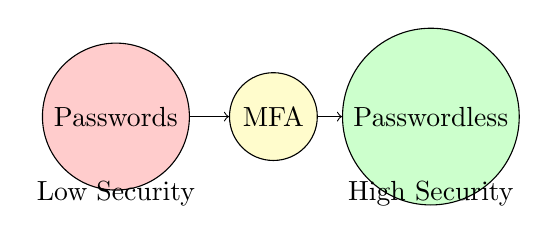
\begin{tikzpicture}
            \node[draw, circle, fill=red!20] (a) at (0,0) {Passwords};
            \node[draw, circle, fill=yellow!20] (b) at (2,0) {MFA};
            \node[draw, circle, fill=green!20] (c) at (4,0) {Passwordless};
            
            \draw[->] (a) -- (b);
            \draw[->] (b) -- (c);
            
            \node[below] at (0,-0.7) {Low Security};
            \node[below] at (4,-0.7) {High Security};
        \end{tikzpicture}
    \end{center}
\end{frame}

\begin{frame}{Multifactor Authentication: Beyond the Password}
    \begin{itemize}
        \item \textbf{Multifactor authentication (MFA)} requires users to provide two or more verification factors to gain access to a resource.
        \item MFA significantly reduces the risk of unauthorized access even if one authentication factor is compromised.
        \item The security benefit of MFA comes from requiring attackers to compromise multiple independent verification methods.
        \item Organizations can implement MFA with varying levels of strictness depending on risk tolerance and usability requirements.
    \end{itemize}
    
    \begin{block}{MFA Implementation Options}
        \begin{itemize}
            \item Required for all users and all access
            \item Required for sensitive operations only
            \item Required based on risk factors (new device, unusual location)
            \item Required for specific user roles or resource types
        \end{itemize}
    \end{block}
\end{frame}

\begin{frame}{Something You Know, Have, Are, or Where You Are: The Four Factors}
    \begin{itemize}
        \item Authentication factors are categorized by the type of verification they provide, with each category offering different security properties.
        \item \textbf{Something you know} includes passwords, PINs, and security questions that rely on secret knowledge.
        \item \textbf{Something you have} includes physical devices like phones, smart cards, or security keys that must be in the user's possession.
        \item \textbf{Something you are} includes biometric characteristics like fingerprints or facial features that are unique to the individual.
        \item \textbf{Somewhere you are} uses location data to verify that access attempts come from expected or approved locations.
    \end{itemize}
    
    \begin{example}
        Withdrawing money from an ATM typically uses two-factor authentication: something you have (the bank card) and something you know (the PIN).
    \end{example}
\end{frame}

\begin{frame}{Biometrics in Action: Using Physical Traits for Authentication}
    \begin{itemize}
        \item \textbf{Biometric authentication} uses unique physical or behavioral characteristics to verify a person's identity.
        \item Common biometric methods include fingerprint scanning, facial recognition, iris scanning, and voice recognition.
        \item Biometrics offer convenience because they don't need to be remembered and are difficult to transfer between individuals.
        \item Unlike passwords, biometric characteristics cannot be changed if compromised, creating unique security challenges.
    \end{itemize}
    
    \begin{table}
        \scriptsize
        \begin{tabular}{|l|l|l|}
            \hline
            \textbf{Biometric Type} & \textbf{Advantages} & \textbf{Limitations} \\
            \hline
            Fingerprint & Fast, accurate, widely accepted & Can be affected by injuries \\
            Facial recognition & Non-intrusive, improving rapidly & Sensitive to lighting, aging \\
            Voice recognition & Works remotely by phone & Background noise, illness affects \\
            Iris scanning & Extremely accurate, stable & Specialized equipment needed \\
            \hline
        \end{tabular}
    \end{table}
\end{frame}

\begin{frame}{Authentication Tokens and Security Keys: Physical Security Tools}
    \begin{itemize}
        \item \textbf{Authentication tokens} generate temporary codes or cryptographic responses that prove the user possesses the token.
        \item \textbf{Hard tokens} are physical devices dedicated to authentication, while \textbf{soft tokens} are software implementations on general-purpose devices.
        \item Time-based One-Time Password (TOTP) tokens generate codes that change periodically and become invalid after a short time.
        \item \textbf{Security keys} like FIDO U2F devices use cryptographic challenges and responses that protect against phishing attacks.
    \end{itemize}
    
    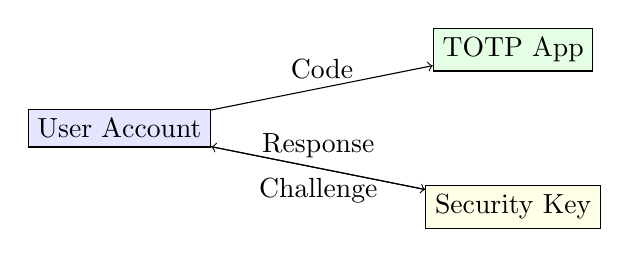
\begin{tikzpicture}
        \node[draw, rectangle, fill=blue!10] (a) at (0,0) {User Account};
        \node[draw, rectangle, fill=green!10] (b) at (5,1) {TOTP App};
        \node[draw, rectangle, fill=yellow!10] (c) at (5,-1) {Security Key};
        
        \draw[->] (a) -- (b) node[midway, above] {Code};
        \draw[->] (a) -- (c) node[midway, below] {Challenge};
        \draw[->] (c) -- (a) node[midway, above] {Response};
    \end{tikzpicture}
\end{frame}

\begin{frame}{Federation: Extending Trust Across Organizations}
    \begin{itemize}
        \item \textbf{Identity federation} allows organizations to recognize and accept identity credentials issued by trusted external parties.
        \item Federation establishes trust relationships that enable secure authentication across organizational boundaries without duplicate accounts.
        \item In federated systems, users authenticate with their home organization (identity provider) to access resources at partner organizations (service providers).
        \item Federation reduces administrative overhead while improving security by centralizing identity management.
    \end{itemize}
    
    \begin{center}
        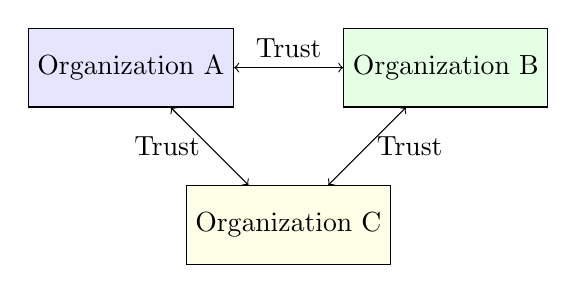
\begin{tikzpicture}
            \node[draw, rectangle, fill=blue!10, minimum width=2cm, minimum height=1cm] (a) at (0,0) {Organization A};
            \node[draw, rectangle, fill=green!10, minimum width=2cm, minimum height=1cm] (b) at (4,0) {Organization B};
            \node[draw, rectangle, fill=yellow!10, minimum width=2cm, minimum height=1cm] (c) at (2,-2) {Organization C};
            
            \draw[<->] (a) -- (b) node[midway, above] {Trust};
            \draw[<->] (b) -- (c) node[midway, right] {Trust};
            \draw[<->] (a) -- (c) node[midway, left] {Trust};
        \end{tikzpicture}
    \end{center}
\end{frame}

\begin{frame}{Single Sign-On: One Key for Many Doors}
    \begin{itemize}
        \item \textbf{Single Sign-On (SSO)} allows users to authenticate once and gain access to multiple systems without re-entering credentials.
        \item SSO improves user experience by eliminating the need to remember and manage multiple sets of credentials.
        \item From a security perspective, SSO reduces password fatigue and encourages stronger authentication for the single login point.
        \item SSO can be implemented within a single organization (enterprise SSO) or across multiple organizations (federated SSO).
    \end{itemize}
    
    \begin{alertblock}{Security Consideration}
        While SSO is generally more secure, it creates a single point of failure - if the SSO account is compromised, all connected applications are potentially vulnerable.
    \end{alertblock}
\end{frame}

\begin{frame}{LDAP, OAuth, and SAML: Understanding Authentication Protocols}
    \begin{itemize}
        \item \textbf{Lightweight Directory Access Protocol (LDAP)} is a protocol for accessing and maintaining directory information services.
        \item LDAP servers store user accounts and authentication information in a hierarchical directory structure for organizational use.
        \item \textbf{Security Assertion Markup Language (SAML)} is an XML-based standard for exchanging authentication and authorization data between parties.
        \item \textbf{Open Authorization (OAuth)} enables third-party applications to obtain limited access to user accounts without sharing credentials.
    \end{itemize}
    
    \begin{table}
        \begin{tabular}{|l|l|}
            \hline
            \textbf{Protocol} & \textbf{Primary Use Case} \\
            \hline
            LDAP & Directory services within organizations \\
            SAML & Enterprise SSO and cross-domain federation \\
            OAuth & Delegated authorization for third-party applications \\
            OpenID Connect & User authentication based on OAuth 2.0 \\
            \hline
        \end{tabular}
    \end{table}
\end{frame}

\begin{frame}{Interoperability: Making Different Systems Work Together}
    \begin{itemize}
        \item \textbf{Interoperability} refers to the ability of different IAM systems to work together seamlessly despite differences in design and implementation.
        \item Standards-based approaches ensure consistent interpretation of identity information across heterogeneous systems.
        \item \textbf{Attestation} provides verified claims about identity attributes that can be trusted across organizational boundaries.
        \item Modern IAM systems must balance proprietary features with compatibility with widely-adopted industry standards.
    \end{itemize}
    
    \begin{block}{Key Interoperability Standards}
        \begin{itemize}
            \item SCIM (System for Cross-domain Identity Management) for user provisioning
            \item JWT (JSON Web Tokens) for securely transmitting claims between parties
            \item X.509 certificates for public key infrastructure
            \item FIDO (Fast Identity Online) for passwordless authentication
        \end{itemize}
    \end{block}
\end{frame}

\begin{frame}{Privileged Access: Managing the Keys to the Kingdom}
    \begin{itemize}
        \item \textbf{Privileged access} refers to elevated permissions that provide extensive control over critical systems and sensitive data.
        \item Privileged accounts represent the highest security risk because they can bypass normal security controls and make widespread changes.
        \item \textbf{Privileged Access Management (PAM)} includes special controls to secure, monitor, and audit privileged account usage.
        \item Effective PAM requires both technical solutions and operational practices like separation of duties and regular access reviews.
    \end{itemize}
    
    \begin{example}
        Examples of privileged accounts include domain administrators, database administrators, root accounts on servers, emergency access accounts, and service accounts that run critical system processes.
    \end{example}
\end{frame}

\begin{frame}{Just-in-Time Permissions: Access When Needed}
    \begin{itemize}
        \item \textbf{Just-in-Time (JIT) permissions} provide elevated access only when needed and only for the duration required.
        \item JIT permissions reduce the risk of privilege abuse by limiting the window of opportunity for malicious actions.
        \item Implementation typically involves a workflow where users request temporary privileges with justification and receive automatic expiration.
        \item This approach follows the principle of zero standing privileges, where no user permanently holds administrative rights.
    \end{itemize}
    
    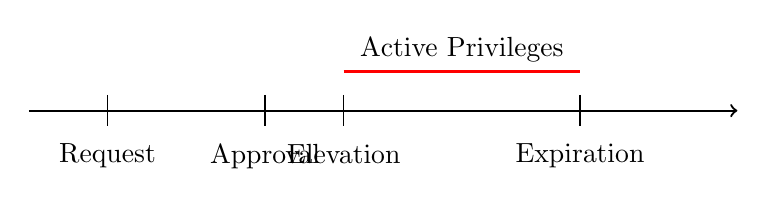
\begin{tikzpicture}
        \draw[->, thick] (0,0) -- (9,0);
        
        \draw (1,0.2) -- (1,-0.2);
        \node[below] at (1,-0.3) {Request};
        
        \draw (3,0.2) -- (3,-0.2);
        \node[below] at (3,-0.3) {Approval};
        
        \draw (4,0.2) -- (4,-0.2);
        \node[below] at (4,-0.3) {Elevation};
        
        \draw (7,0.2) -- (7,-0.2);
        \node[below] at (7,-0.3) {Expiration};
        
        \draw[-, very thick, red] (4,0.5) -- (7,0.5);
        \node[above] at (5.5,0.5) {Active Privileges};
    \end{tikzpicture}
\end{frame}

\begin{frame}{Password Vaulting and Ephemeral Credentials: Temporary Access Solutions}
    \begin{itemize}
        \item A \textbf{password vault} securely stores privileged account credentials and controls their usage through check-out procedures and automatic rotation.
        \item Password vaults eliminate the need for users to know actual passwords while still allowing controlled access to privileged accounts.
        \item \textbf{Ephemeral credentials} are temporary authentication secrets generated for a single session and discarded afterward.
        \item Cloud environments increasingly use ephemeral credentials to minimize the risk of long-lived access keys being compromised.
    \end{itemize}
    
    \begin{alertblock}{Security Benefit}
        With properly implemented password vaulting, even administrators cannot access privileged credentials directly, reducing insider threat risks and preventing password sharing among team members.
    \end{alertblock}
\end{frame}

\begin{frame}{IAM Best Practices: Putting It All Together}
    \begin{itemize}
        \item Implement the principle of least privilege by providing minimal access required for each job function.
        \item Use multifactor authentication for all accounts, especially those with privileged access.
        \item Automate provisioning and de-provisioning to ensure consistency and timeliness.
        \item Conduct regular access reviews to identify and correct inappropriate permissions.
    \end{itemize}
    
    \begin{block}{Balancing Security and Usability}
        The most effective IAM implementations find the right balance between:
        \begin{itemize}
            \item Strong security controls without excessive user friction
            \item Centralized governance with appropriate delegation
            \item Standardized policies with flexibility for special cases
            \item Automated processes with human oversight
        \end{itemize}
    \end{block}
\end{frame}

\begin{frame}{The Future of Identity and Access Management: Trends and Challenges}
    \begin{itemize}
        \item The movement toward \textbf{Zero Trust Architecture} emphasizes continuous verification rather than implicit trust based on network location.
        \item \textbf{Artificial intelligence} is increasingly used to detect abnormal access patterns and provide risk-based authentication.
        \item \textbf{Decentralized identity} approaches using blockchain technology promise user control over personal data and credentials.
        \item Cloud and mobile computing continue to challenge traditional perimeter-based security models and drive IAM innovation.
    \end{itemize}
    
    \begin{center}
        \begin{tabular}{|c|c|}
            \hline
            \textbf{Traditional IAM} & \textbf{Future IAM} \\
            \hline
            Static permissions & Dynamic, contextual access \\
            Password-centric & Passwordless authentication \\
            Organization-controlled & User-controlled identity \\
            Perimeter-focused & Zero Trust model \\
            \hline
        \end{tabular}
    \end{center}
\end{frame}

\end{document}